\documentclass{standalone}
\usepackage{pgfplots}
\pgfplotsset{compat=1.17}

\begin{document}

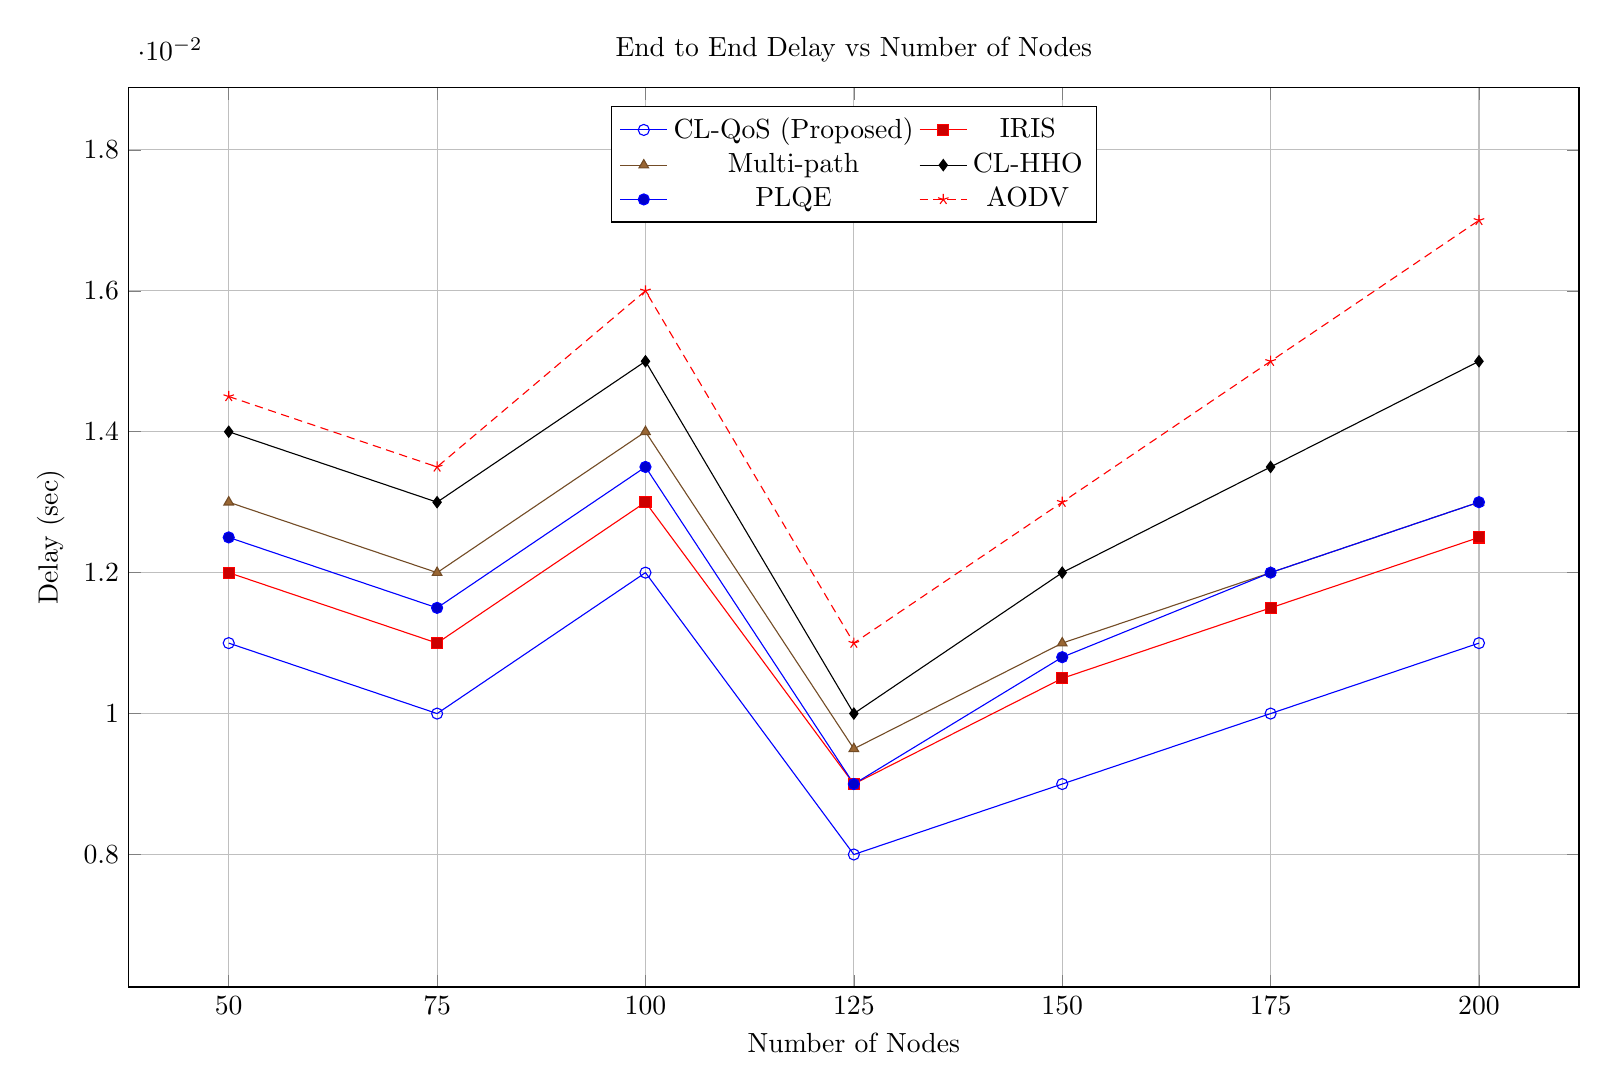
\begin{tikzpicture}

\begin{axis}[
width=20cm,
height=13cm,
title={End to End Delay vs Number of Nodes},
xlabel={Number of Nodes},
ylabel={Delay (sec)},
enlargelimits=0.08,
ymin=0.007, ymax=0.018,
xtick={50,75,100,125,150,175,200},
ytick={0.008,0.010,0.012,0.014,0.016,0.018},
legend columns=2,
legend style={at={(0.5,0.98)},anchor=north},
grid=both
]

% CL-QoS
\addplot+[mark=o] coordinates {
(50,0.011) (75,0.010) (100,0.012) (125,0.008)
(150,0.009) (175,0.010) (200,0.011)
};

% IRIS
\addplot+[mark=square*] coordinates {
(50,0.012) (75,0.011) (100,0.013) (125,0.009)
(150,0.0105) (175,0.0115) (200,0.0125)
};

% Multi-path
\addplot+[mark=triangle*] coordinates {
(50,0.013) (75,0.012) (100,0.014) (125,0.0095)
(150,0.011) (175,0.012) (200,0.013)
};

% CL-HHO
\addplot+[mark=diamond*] coordinates {
(50,0.014) (75,0.013) (100,0.015) (125,0.010)
(150,0.012) (175,0.0135) (200,0.015)
};

% PLQE
\addplot+[mark=*] coordinates {
(50,0.0125) (75,0.0115) (100,0.0135) (125,0.009)
(150,0.0108) (175,0.012) (200,0.013)
};

% AODV
\addplot+[mark=star] coordinates {
(50,0.0145) (75,0.0135) (100,0.016) (125,0.011)
(150,0.013) (175,0.015) (200,0.017)
};

\legend{CL-QoS (Proposed), IRIS, Multi-path, CL-HHO, PLQE, AODV}

\end{axis}

\end{tikzpicture}

\end{document}